\newcommand{\psd}[1]{{\small\sffamily{\color{blue!60}#1}}}

Similar simulation, as in the prvious tutorial is presented in this
section. We showcase the 2D bar problem simulation with one end clamped
wile being pulled at the other end. Just like the previous simulation
the body force is neglected, However now the non clamped ends pull is
approximated with Neumann force
\(\int_{\partial\Omega^h_{\text N}}(\mathbf t \cdot \mathbf{v}^h)\). To
simulate the pull we assume traction vector
\(\mathbf t=[t_x,t_y]=[10^9.,0]\) acting on the non clamped right end of
the bar, i.e., force in \(x\) direction is 10 units. Here is how PSD
simulation of this case can be performed.

\textbf{Step 1: Preprocessing}

For ``PSD preprocessing'' go to any folder, launch the terminal there
and run the following command.

\begin{lstlisting}[style=BashInputStyle]
PSD_PreProcess -problem linear-elasticity -dimension 2 -dirichletconditions 1 -tractionconditions 1 -postprocess u
\end{lstlisting}

the comandline flag \psd{ -dirichletconditions 1}, notifies to PSD that
there is one Dirichlet border ---the clamped end of the bar--- in this
simulation. And the flag \psd{ -tractionconditions 1} notifies to PSD
that there is one traction border ---the right end of the bar--- in this
simulation. To provide the clamped boundary condition (\(u_1=0,u_2=0\))
set the variables \psd{ Dbc0On 2}, \psd{ Dbc0Ux 0.}, and
\psd{ Dbc0Uy 0.} in \psd{ ControlParameters.edp}. In the same file
traction boundary conditions are provided via the variables
\psd{ Tbc0On 4} and \psd{ Tbc0Tx 1.e9}, which mean apply traction force
\(\mathbf t=[t_x,t_y]=[10^9.,0]\) on label number 4 (right) of the mesh.
If user wishes to add traction force ,for instance \(t_y=100.\), simply
add the missing macro \psd{ macro Tbc0Tx 1.e9 //}.

\textbf{Step 2: Solving}

Let us now use 5 cores to solve this problem. To do so enter the
following command:

\begin{lstlisting}[style=BashInputStyle]
PSD_Solve -np 5 Main.edp
\end{lstlisting}

Notice, that this is the exact same command used in solving the previous
bar problems from other sections, with only difference that we now use
\psd{ -np 5}.

\textbf{Step 3: Postprocessing}

Launch ParaView and have a look at the \psd{ .pvd} file in the
\psd{ PSD/Solver/VTUs\_DATE\_TIME} folder.

\begin{figure}[htbp]
    \centering
    \begin{minipage}[t][2cm][t]{0.36\textwidth}
    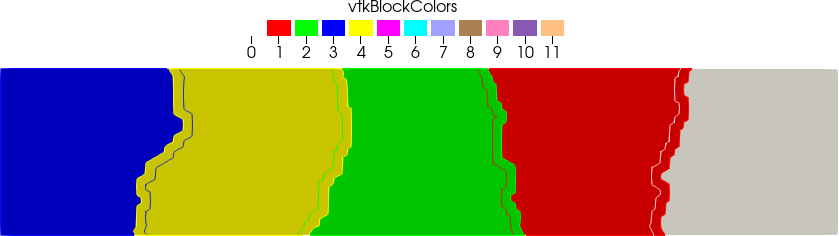
\includegraphics[align=b,width=1\textwidth]{./Images/2d-bar-partitioned5.png}
    \end{minipage}\hspace{.1\textwidth}
    \begin{minipage}[t][2cm][t]{0.5\textwidth}
    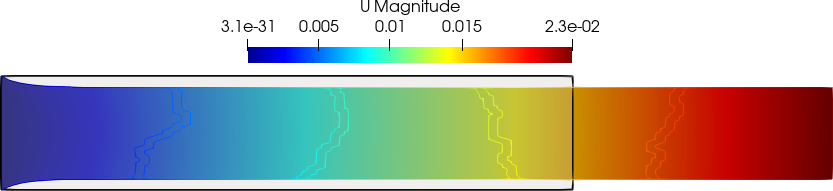
\includegraphics[align=b,width=1\textwidth]{./Images/2d-bar-clamped-traction.png}
    \end{minipage}
    \caption{2D bar results. Partitioned mesh (left) and 100X warped displacement field (right).}
    \label{fig:5part}
\end{figure}

Note now in\textasciitilde{}\ref{fig:5part} there are five subdomains in
the partitioned mesh since five cores were used. Contrary to previous
tutorial, as expected, we see that the right end of the bar which is
being pulled now contract in \(y\) direction. This is due to the fact
that there is no Dirichlet condition at this end now.
